Predictions made by statistical models, scientific applications, and data extraction from unstructured text are well known sources of uncertain data.  Measurements have error margins while predictions are typically drawn from well known distributions.  Traditional database management systems (DBMS) are ill-equipped to manage this kind of uncertainty.  For example, consider a risk-management application that uses statistical models to evaluate the long term effects of corporate decisions and policies.  This application may use a DBMS to store predictions and statistical measures (e.g., error bounds) of those predictions.  However, arbitrary queries made on the predictions do not translate naturally into queries on the corresponding statistical measures.  A user who requires error bounds on the sum of a join over several tables of predictions must first obtain a formula for computing those bounds, assuming a closed form formula even exists.

Probabilistic  database  management  systems \cite{dalvi07efficient, WidomTrio2008, KochMayBMS2008, SD2007, ORION, MCDB, BayesStore} aim at providing better support for querying uncertain data.  Queries in these systems preserve the statistical properties of the data being queried, allowing users to obtain metrics about and representations of query results.  The previously mentioned risk-management application, built on top of a probabilistic database, could use the database itself to obtain error bounds on the results of arbitrary queries over its predictions.  By encoding the statistical model for its predictions in the database itself, the risk-management application could even use the probabilistic database to estimate complex functions over many correlated variables in its model.  In effect, the application could compute all of its predictions within the probabilistic database in the first place.

Few systems are general enough to efficiently query probabilistic data defined over both discrete and continuous distributions.  Those that are, generally rely on sampling to estimate desired values, as exact solutions can be hard to obtain.  If a query contains a selection predicate, samples violating the predicate are dropped and do not contribute to the expectation.  The more selective the predicate, the more samples are needed to maintain consistent accuracy.  For example, a query may combine a model predicting customer profits with a model for predicting dissatisfied customers, perhaps as a result of a corporate decision to use a cheaper, but slower shipping company.  If the query asks for profit loss due to dissatisfied customers, the query need only consider profit from customers under those conditions where the customer is dissatisfied (ie, the underlying model may include a correlation between ordering patterns and dependence on fast shipping).  

Without knowing the likelihood that customer A is satisfied, the query engine must over-provision and waste time generating large numbers of samples, or risk needing to re-evaluate the query if additional samples are needed.  This problem is well known in online aggregation, but ignored in general-purpose (i.e., both discrete and continuous) probabilistic databases.  

Selective queries exemplify the need for contextual information when computing expectations and moments.  This paper presents PIP, a highly extensible, general probabilistic database system built around this need for information.  PIP evaluates queries on symbolic representations of probabilistic data, making a complete representation of the expression to be evaluated available before an expectation or moment is taken.  To our knowledge, PIP is the first probabilistic database system supporting continuous distributions to evaluate queries in this way.

\subsection{Symbolic Representation}
Representing the uncertain components of a query's output symbolically makes a wide variety of integration techniques available for use in evaluating the statistical characteristics of the expression.  If our risk-management application assumes a general model of customer profit and customer satisfaction that relies on queries to create correlations between them, the sampler can detect this lack of dependency, estimate profit and probability of dissatisfaction separately, and combine the two afterwards.  Even with relatively straightforward integration techniques, additional knowledge of this form has a profoundly positive impact on the efficiency and accuracy with which expectations of query results can be computed.

Accuracy is especially relevant in cases where the integral has no closed form and exact methods are unavailable.  This is the case in a surprising range of practical applications, even when strong simplifying assumptions are made about the input data.  For example, even if the input data contains only independent variables sampled from well-studied distributions (e.g., the normal distribution), it is still possible for queries to create complex statistical dependencies in their own right.  It is well known, at least in the case of discrete and finite probability distributions, that relational algebra on block-independent-disjoint tables can construct any finite probability distribution\ \cite{1325861,IL1984}.

%

\begin{figure}[!]
\begin{center}
\begin{tabular}{rc}
& Query
\\
%\\
%\hline
\\
\begin{tabular}{r}
query \\
evaluation
\end{tabular}
&
\framebox{
\begin{tabular}{c}
\framebox{
\begin{tabular}{p{4.2cm}}
computing probabilities, \\
moments, and statistical tests
\end{tabular}
}
\\[3ex]
\framebox{
\begin{tabular}{p{4.2cm}}
query plans on c-tables
\end{tabular}
}
\end{tabular}
}
\\[7ex]
\begin{tabular}{l}
data \\
store
\end{tabular}
&
\framebox{
\begin{tabular}{c}
\framebox{
\begin{tabular}{p{4.2cm}}
(probabilistic) c-tables
\end{tabular}
}
\\[2ex]
\framebox{
\begin{tabular}{p{4.2cm}}
succinct representation of \\
joint distribution of random \\
variables (exchangeable)
\end{tabular}
}
\end{tabular}
}
\end{tabular}
\end{center}
\caption{Pip Query Engine Architecture.}
\label{fig:arch}
\end{figure}



\begin{figure}
\begin{center}
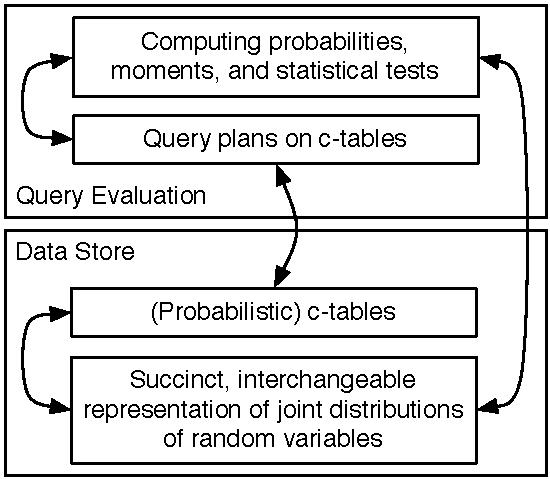
\includegraphics[width=2in]{graphics/arch.pdf}
\vspace*{-0.1in}
\caption{Pip Query Engine Architecture}
\label{fig:arch}
\end{center}
\vspace*{-0.35in}
\end{figure}

PIP represents probabilistic data values symbolically via random variables defined in terms of parametrized probability distribution classes.  PIP supports several generic classes of probability distributions (e.g., Normal, Exponential, Poisson), and may be extended with additional classes.  Variables are treated as opaque while they are manipulated by traditional relational operators.  The result is a symbolic representation of uncertainty, a c-table \cite{IL1984,GT2006, KochMayBMS2008}.  As the final stage of the query, special operators defined within PIP compute expectations and moments of the uncertain data, or sample the data to generate histograms.  

These expectation operators are invoked with an unbiased, lossless representation of the expression to be evaluated.  Because the variables have been treated as opaque, the expectation operator can obtain information about the distribution a variable corresponds to.  Developers can (but need not) provide supplemental information (e.g., functions defining the PDF and the CDF) about distributions they extend PIP with.  The operator can exploit this additional information to accelerate the sampling process, or potentially even sidestep it entirely.  For example, if a query asks for the probability that a variable will fall within specified bounds, the expectation operator can compute it with at most two evaluations of the variable's CDF.

Because the symbolic representation PIP uses is lossless, intermediate query results or views may be materialized.  Expectations of values in these views or subsequent queries based on them will not be biased by estimation errors introduced by materializing the view.  This is especially useful when a significant fraction of query processing time is devoted to managing deterministic data (eg, to obtain parameters for the model's variables).  Not only can this accelerate processing of commonly used subqueries, but it makes online sampling feasible; the sampler need not evaluate the entire query from scratch to generate additional samples.


\begin{example}\em
\label{ex:intro}
Suppose a database captures customer orders expected for the next quarter,
including prices
and destinations of shipment. The order prices are 
uncertain, but a probability distribution is assumed.
The database also stores
distributions of shipping durations for each location.
Here are two c-tables defining such a probabilistic database:
\[
\begin{tabular}{c|ccc}
Order & Cust & ShipTo & Price \\
\hline
& Joe & NY & $X_1$ \\
& Bob & LA & $X_3$ \\
\end{tabular}
%\hspace{5mm}
\]\[
\begin{tabular}{c|cc}
Shipping & Dest & Duration \\
\hline
& NY & $X_2$ \\
& LA & $X_4$ \\
\end{tabular}
\]
We assume a suitable specification of the joint distribution $p$ of the random
variables $X_1,\dots,X_4$ occurring in this database.

Now consider the query
\begin{verbatim}
select expected_sum(O.Price)
from   Order O, Shipping S
where  O.ShipTo = S.Dest
and    O.Cust = 'Joe'
and    S.Duration >= 7;
\end{verbatim}
asking for the expected loss due to late deliveries to customers named Joe,
where the product is free if not delivered within seven days.
%
This can be approximated by drawing a number of samples from $p$
and using formula~\ref{eq:mc_expectation}
to approximate $E[q]$,
where $q$ represents the result of the sum aggregate query on a sample,
here
\[
q(\vec{x}) =
\left\{
\begin{array}{lll}
x_1 & \dots & x_2 \ge 7 \\
0 & \dots & \mbox{otherwise.}
\end{array}
\right.
\]

In a naive sample-first approach, 
if $x_2 \ge 7$ is a relatively rare event, a large number of samples will be
required to compute a good approximation to the expectation.
Moreover, the profit $x_1$ is independent from the shipping time $x_2$.  Despite this, samples for $x_1$ are still discarded if the constraint on $x_2$ is not met.

Now consider using c-tables. The result of the relational algebra part of the
above query can be easily computed as
\[
\begin{tabular}{c|c|c}
R & Price & Condition \\
\hline
& $X_1$ & $X_2 \ge 7$ \\
\end{tabular}
\]
without looking at $p$.
This c-table compactly represents all data still relevant after the
application of the relational algebra part of the query, other than $p$,
which remains unchanged.
Sampling from R to compute
\begin{verbatim}
select expected_sum(Price) from R;
\end{verbatim}
is a much more focused effort.
First, we only have to consider the random variables relating to Joe;
but determining that random variable $X_2$ is relevant while $X_4$
is not requires
executing a query involving a join. We want to do this query first, before
we start sampling.

Second, assume that delivery times are
independent from sales volumes. Then we can approximate the
query result
by first sampling an $X_2$ value and only sampling an $X_1$ value if $X_2 \ge 7$.
Otherwise, we use $0$ as the $X_1$ value.
If $X_2 \ge 7$ is relatively rare (e.g., the average shipping times to NY are
very slow, with a low variance), this may reduce the amount of samples
for $X_1$ that are first computed and then discarded without seeing use
considerably.
If CDFs are available, we can of course do even better.
%
\end{example}

\subsection{Background and Related Work}
There is one conceptually simple technique, however, that  allows for the (approximate) numerical integration of even  the most general  functions, including those occurring in  probabilistic data  processing: Monte Carlo integration \cite{montecarlo}. Conceptually, to compute an expectation, one simply approximates   the  integral  by  taking $n$ samples $\vec{x}_1, \dots, \vec{x}_n$ for $\vec{X}$ from $p$  and  taking  the  average of the $q$ values,
%
\begin{equation}\label{eq:mc_expectation}
\frac{1}{n} \cdot \sum_{i=1}^n q(\vec{x}_i).
\end{equation}

In general, even taking a sample from a complicated PDF is difficult.  Constraints imposed by queries break assumptions of normalization on $p(\vec x)$ and require that the sampling technique account for them or lose precision.  A variety of techniques exist to address this problem, from straightforward rejection sampling, where constraint-violating samples are repeatedly discarded, to more heavy duty Markov-chain Monte Carlo (MCMC, cf.\ e.g., \cite{GRS1995}) style techniques such as the Metropolis-Hastings algorithm \cite{metropolis,GRS1995}. 

Recently,  the paper  \cite{MCDB} on  the MCDB  system  has promoted an integrated  sampling-based  approach to  probabilistic databases.  Conceptually,  MCDB uses a {\em sample-first}\/ approach: it   first  computes  samples  of  entire databases and then processes queries  on these samples.  This is a very general and flexible approach, largely due to its modular approach to probability distributions via black box sample generators called VG Functions.  Using Tuple-Bundles, a highly compressed representation of the sampled database instances, MCDB evaluates queries on these instances in parallel, sharing computation across instances where possible.  

{\em  Conditional tables}\/  (c-tables, \cite{IL1984})  are relational tables in which tuples have associated conditions expressed as boolean expressions over  comparisons of random variables  and constants. C-tables are a natural way to  represent  the  {\em  deterministic skeleton}\/  of a probabilistic relational  database in  a succinct  and tabular  form.  That  is, complete information  about uncertain data is encoded using random  variables, excluding only  specifications  of the  joint  probability  distribution of  the random  variables   themselves.   This  model   allows  representation of  input databases  with  nontrivial statistical  dependencies that are normally associated with graphical models. 

For {\em discrete} probabilistic  databases, a canon of systems has been developed that essentially use c-tables, without referring to them as such. MystiQ  \cite{dalvi07efficient}  uses  c-tables internally  for  query processing  but  uses  a  simpler  model for  input  databases.   Trio \cite{WidomTrio2008}  uses  c-tables with  additional  syntactic sugar  and calls conditions {\em lineage}\/.  MayBMS \cite{AJKO2008}  uses a  form of  c-tables called  U-relations that define how relational algebra representations of queries can encode the corresponding condition transformations.

\subsection{Contributions}

The  c-tables  approach has  never  been used  to build  a
probabilistic  database  management  system that  supports  continuous
probability  distributions.
%
ORION \cite{ORION} is a probabilistic database management system for
continuous distributions that can alternate between sampling
and transforming distributions. However, their representation
system is not based on c-tables but essentially on the
world-set decompositions of \cite{AKO07WSD}, a factorization
based approach related to graphical models.
Selection queries in this model may require an exponential blow-up in the
representation size, while selections are efficient in c-tables.


{\em PIP}\/'s approach encompasses and extends the strengths of discrete systems that use c-tables such as MystiQ and MayBMS, as well as the generality of MCDB's Monte-Carlo approach.  It supports both discrete and continuous probability distributions, statistical dependencies definable by queries, expectations of aggregates and distinct-aggregates with or without  group-by,  and the computation of confidences. The detailed technical contributions of this paper are as follows.


\begin{itemize}
\addtolength{\topsep}{-0.3ex}
\addtolength{\labelsep}{-0.3ex}
\addtolength{\itemsep}{-1ex}
\item
We study query evaluation using probabilistic conditional tables, for
relational algebra, aggregates, and the computation of expectations and
probabilities.

\item
We present the architectural and language design decisions made in the
PIP system, and show how the various techniques introduced combine into
a unified whole.

\item
We provide experimental evidence for the competitiveness of our approach, comparing PIP with a reimplementation of the refined sample-first approach taken by MCDB.  We use a common codebase for both systems based on Postgres to enable fair comparison.  We show that PIP performs considerably better than MCDB over a wide range of queries.  Even in the worst case, PIP remains competitive with MCDB (it essentially never does more work).
\end{itemize}

The structure of this paper is as follows. Section~\ref{sec:background} presents probabilistic c-tables, and the conceptual  evaluation of queries on probabilistic c-tables. Section~\ref{sec:sampling} studies sampling and other mechanisms for computing integrals, and examines how PIP uses and enhances them.  In Section~\ref{sec:design}, we present a high level view of PIP in the abstract.   Section~\ref{sec:implementation} discusses details of the implementation of PIP and our reimplementation of MCDB.  Finally, in Section~\ref{sec:evaluation}, we present the outcomes of our experiments with PIP and our MCDB reimplementation.